%!TEX root = mb.tex
\begin{figure}[t]
  \centering
  \begin{tabular}{cc}
  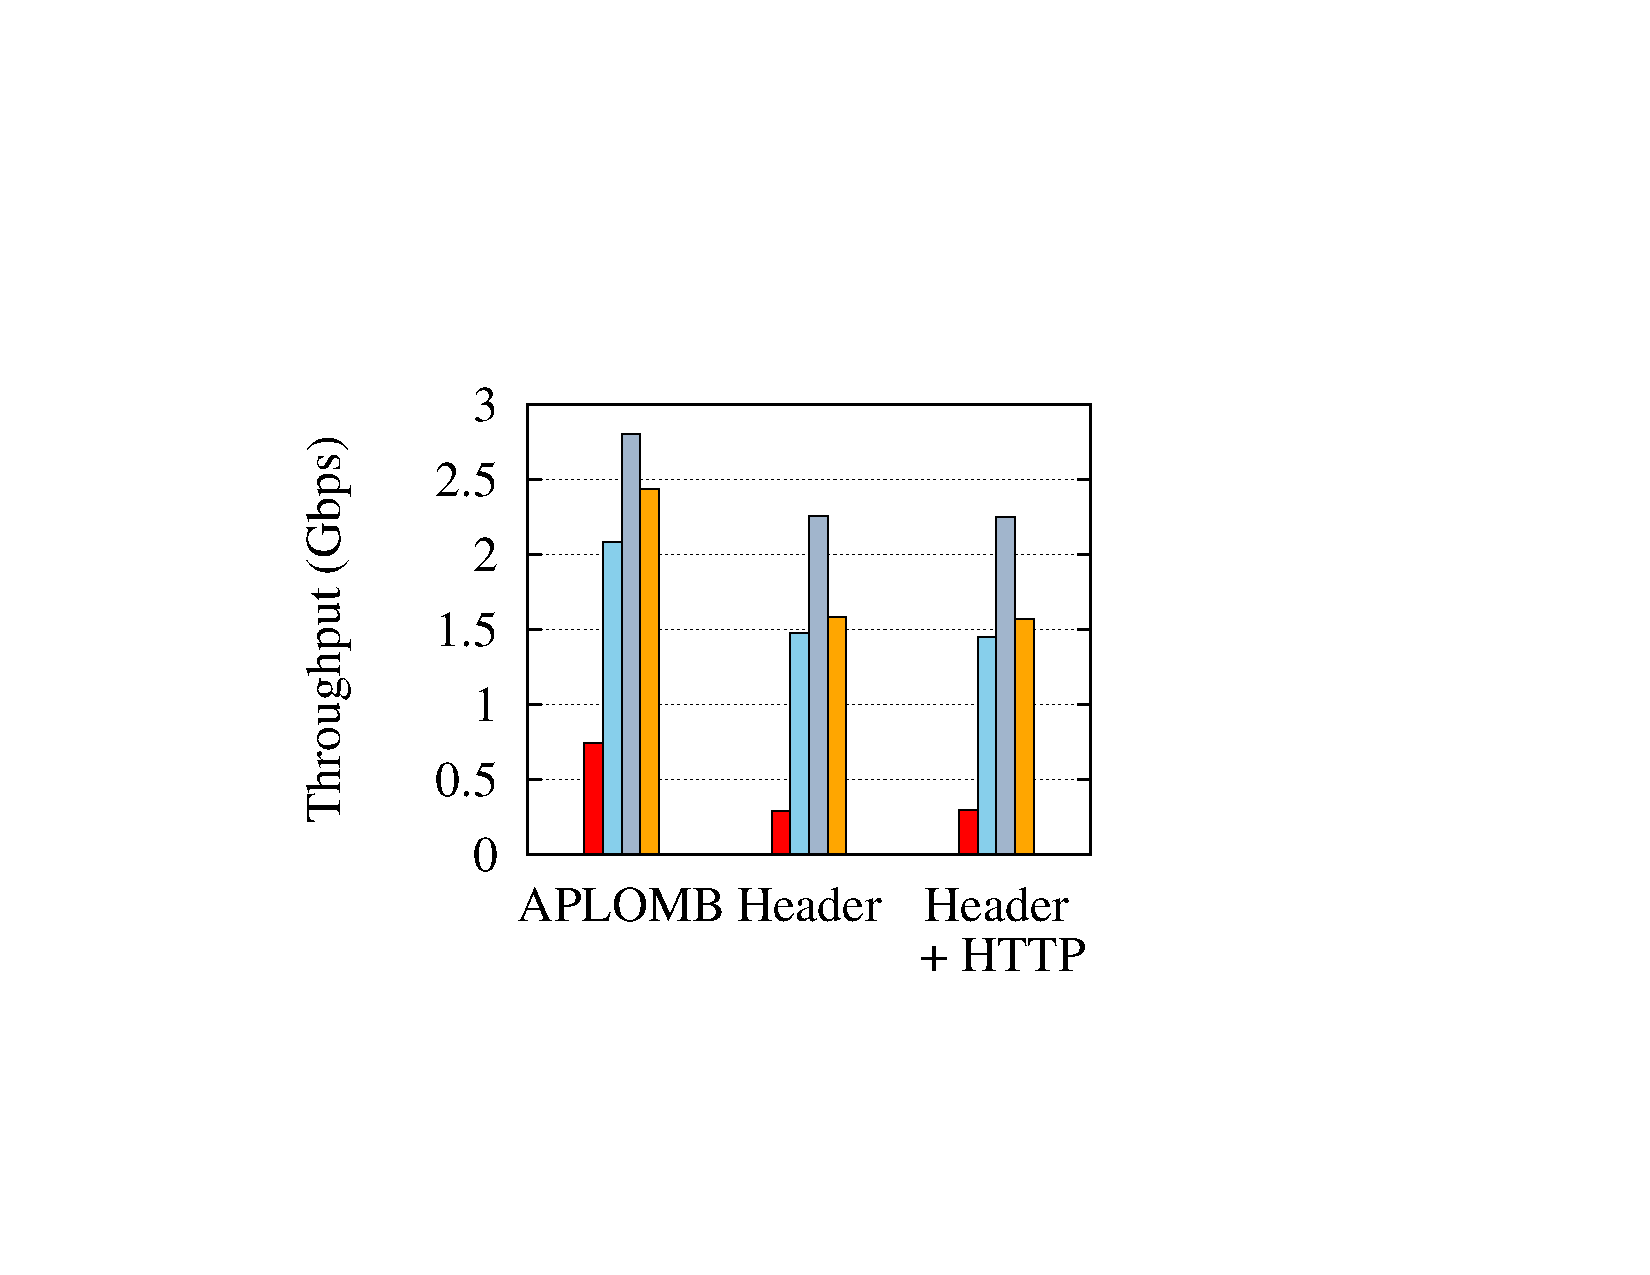
\includegraphics[height=1in]{fig/gateway_xput}&
  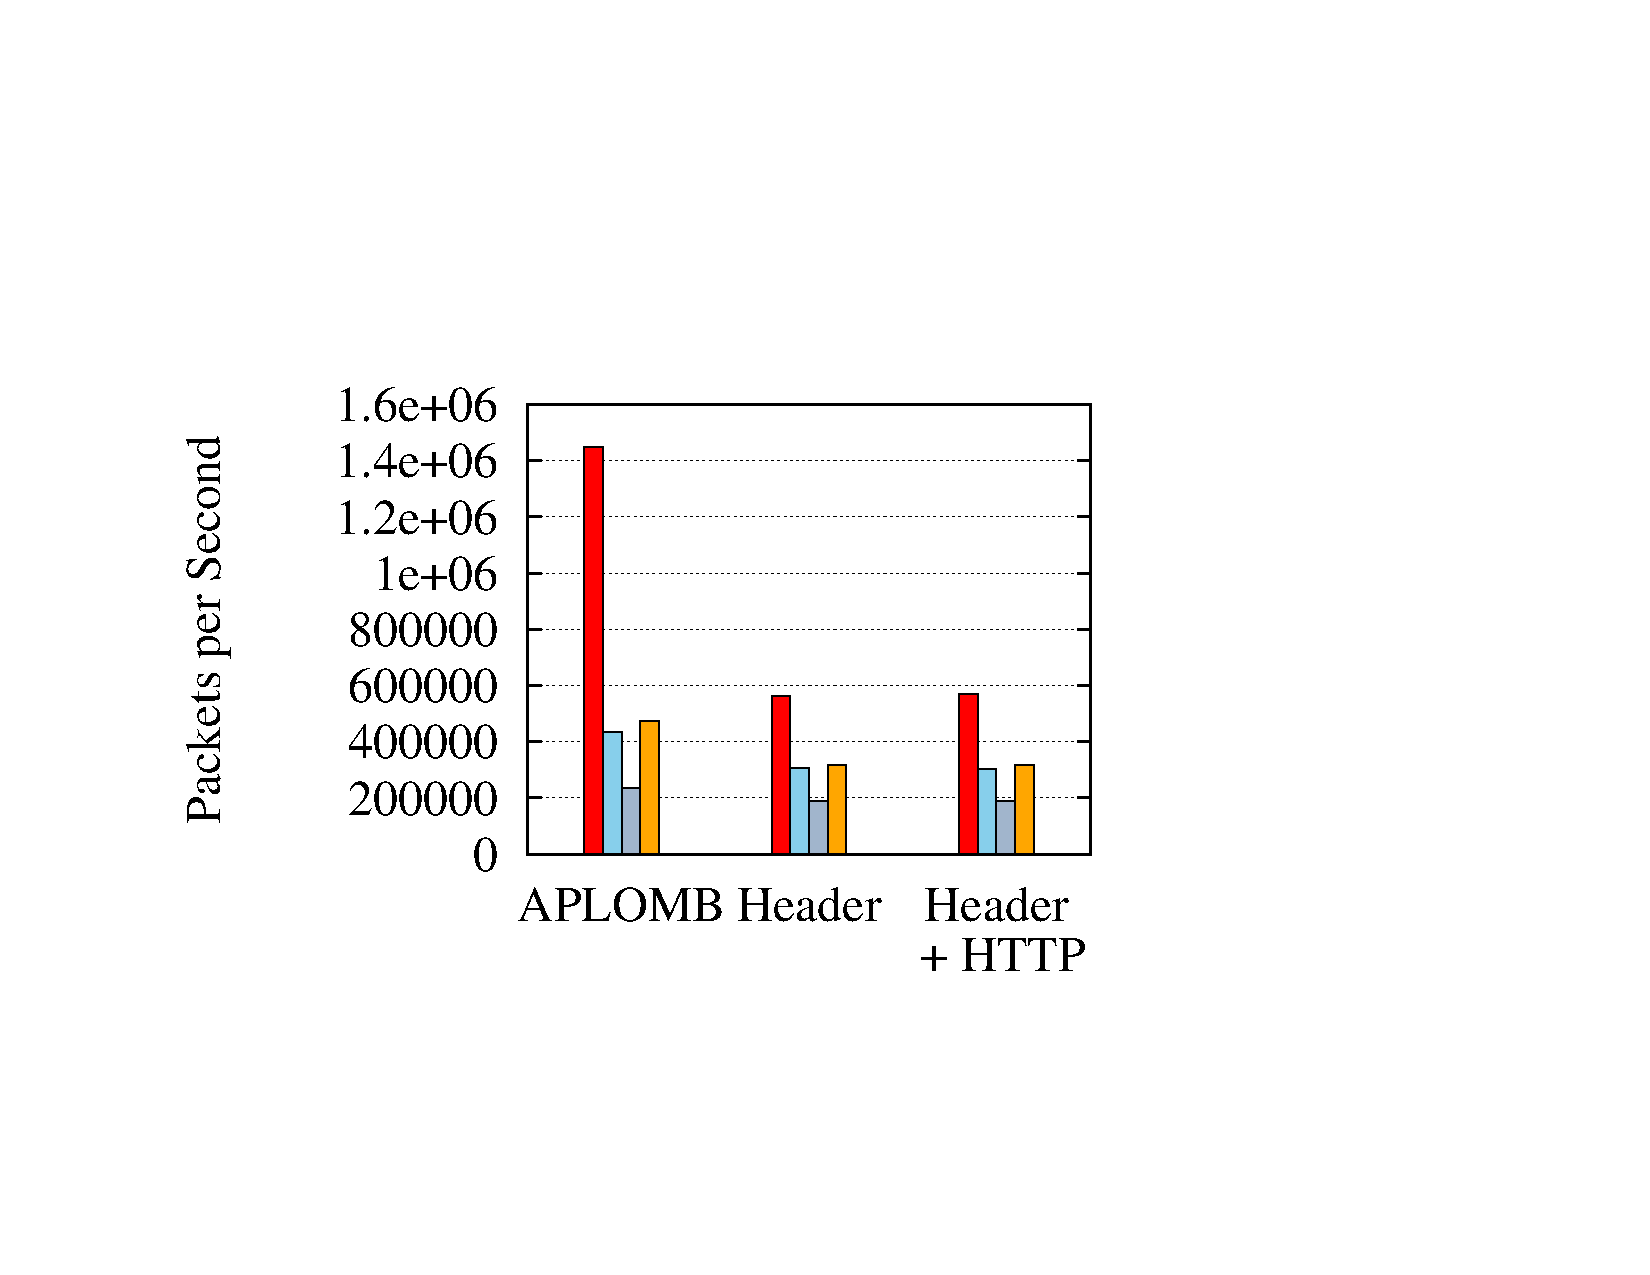
\includegraphics[height=1in]{fig/gateway_pps}\\
  \end{tabular}
  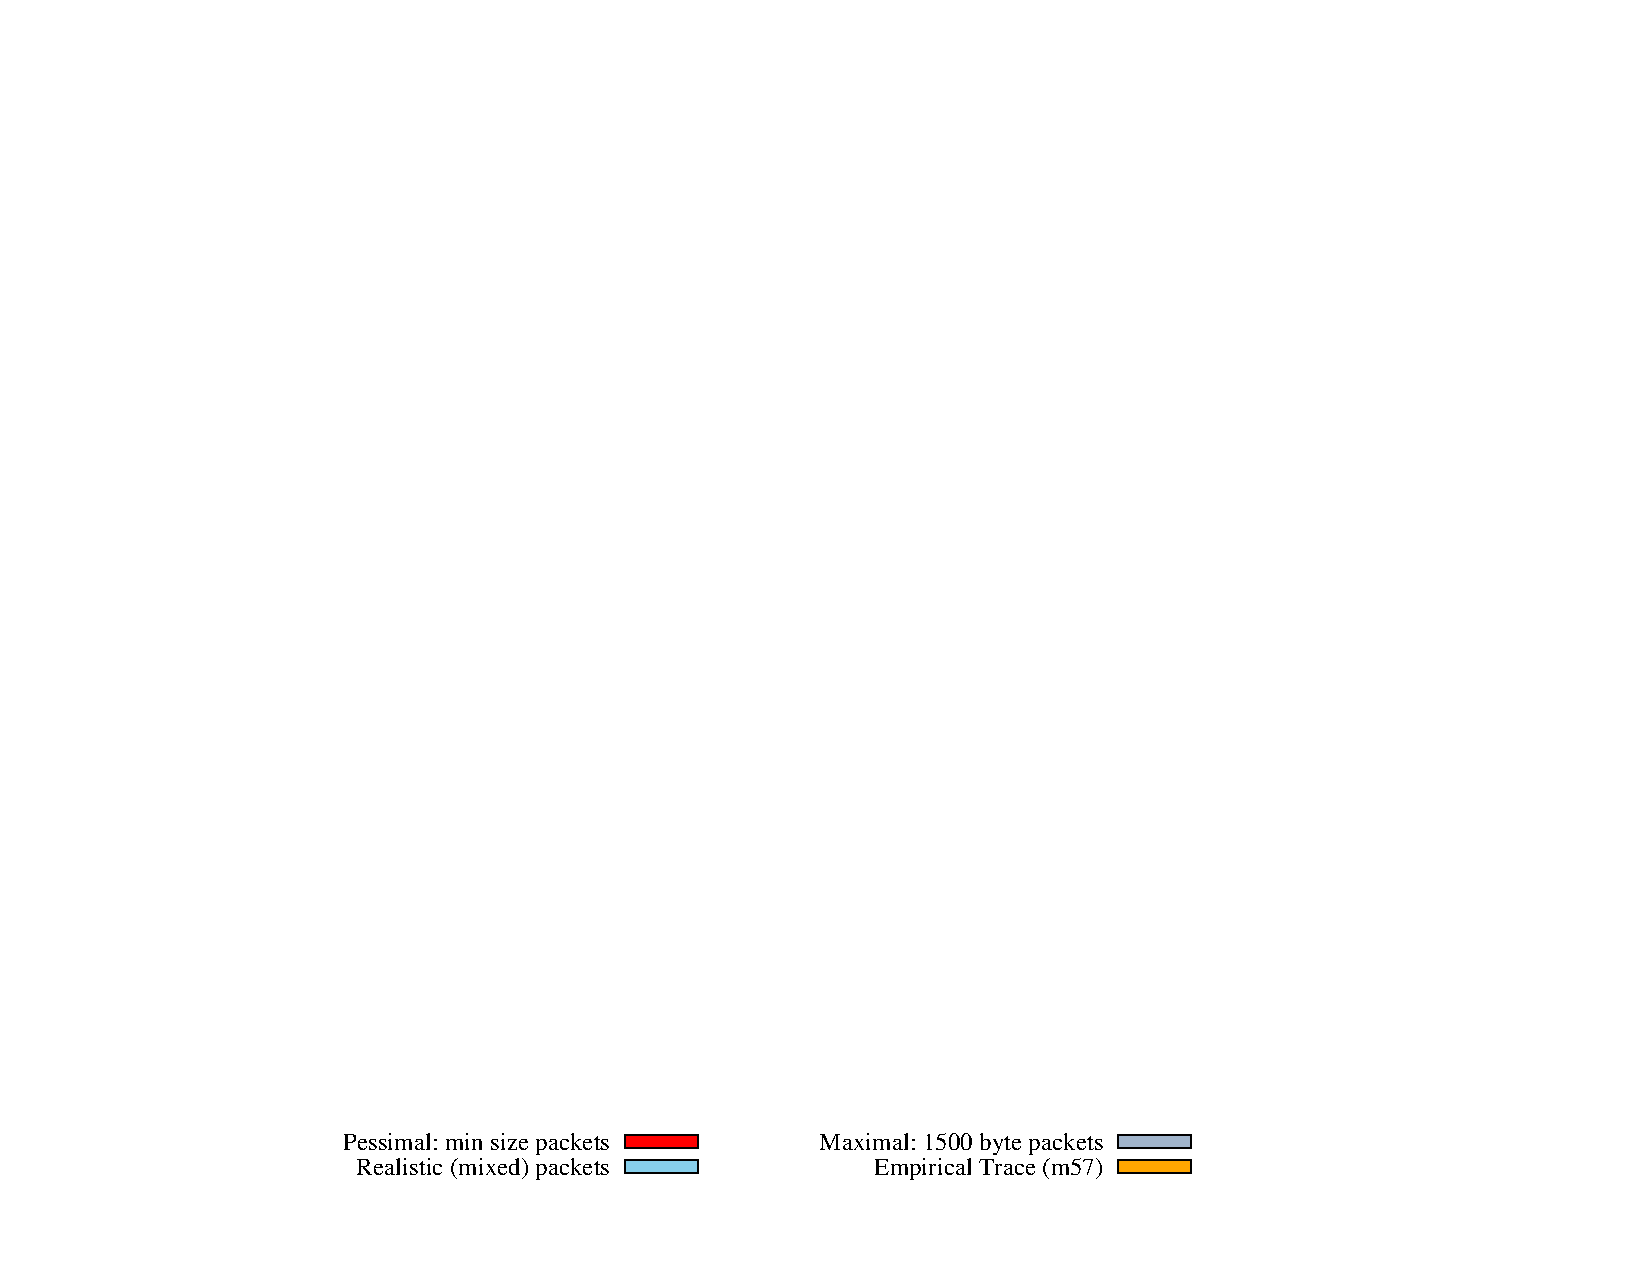
\includegraphics[width=2.75in]{fig/key}
  \caption[]{\label{fig:gwxput} Throughput on a single core at stateless gateway.}
\end{figure}

\begin{figure}[t]
  \centering
  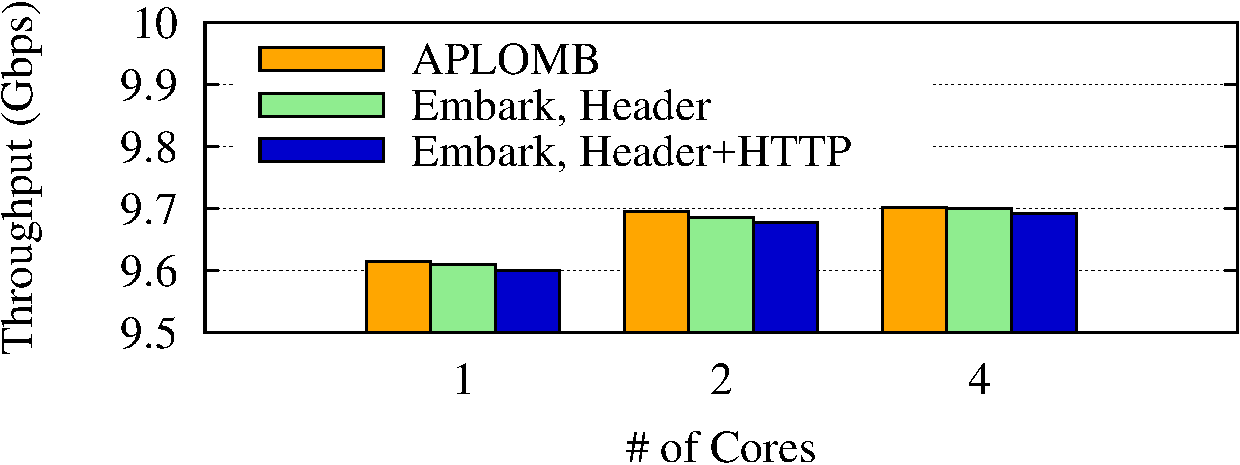
\includegraphics[width=2.8in]{fig/gateway_scale}
  \caption[]{\label{fig:gwscale} Gateway throughput with increasing parallelism.}
\end{figure}
 
\section{Evaluation} \label{sec:eval}

As we showed in \S\ref{sec:mbs}, \sys supports all middlebox applications in typical outsourcing environments~\cite{aplomb,etsi-nfv}. Hence, from a functionality perspective, \sys answers our original question, ``Is it possible to enable a third party to perform traffic processing for an enterprise, {\em without seeing the enterprise's traffic}?''  in the affirmative.

We now investigate whether \sys is practical from a performance perspective, looking at the overheads due to encryption and redirection. 
We built our gateway using Click~\cite{click} over DPDK~\cite{dpdk} on an off-the-shelf 16-core server with 2.6GHz Xeon E5-2650 cores and 128GB RAM; the network hardware is a single 10GbE Intel 82599 compatible network card. 
We deployed our prototype gateway in our research lab and redirected traffic from a 3-server testbed through the gateway; these three client servers had the same hardware specifications as the server we used as our gateway.
We deployed our middleboxes on Amazon EC2.
For most experiments, we use a synthetic workload generated by the Pktgen~\cite{pktgen}; for experiments where an empirical trace is specified we use the m57 patents trace~\cite{m57} and the ICTF 2010 trace~\cite{ictf}, both in IPv4.

%In what follows, we evaluate our performance at the enterprise, including gateway throughput, end-to-end page load times, and bandwidth costs (\S\ref{sec:enterprise}). We then evaluate performance at the cloud, evaluating each middlebox we implemented one by one (\S\ref{sec:evalcloud}).

\subsection{Enterprise Performance}
\label{sec:enterprise}
We first evaluate \sys's overheads at the enterprise. %including the gateway, end-to-end performance, and bandwidth costs from deploying \sys.

\subsubsection{Gateway}

 
\noindent{\it How many servers does a typical enterprise require to outsource traffic to the cloud?}
Figure~\ref{fig:gwxput} shows the gateway throughput when encrypting traffic to send to the cloud, first with normal redirection (as used in APLOMB~\cite{aplomb}), then with \sys's L3/L4-header encryption, and finally with L3/L4-header encryption as well as stateless HTTP/proxy encryption. 
For empirical traffic traces with payload encryption (DPI) disabled, \sys averages 9.6Gbps per core; for full-sized packets it achieves over 9.8Gbps.
In scalability experiments (Fig.~\ref{fig:gwscale}) with 4 cores dedicated to processing, our server could could forward at up to 9.7Gbps for empirical traffic while encrypting for headers and HTTP traffic.
There is little difference between the HTTP overhead and the L3/L4 overhead, as the HTTP encryption only occurs on HTTP requests -- a small fraction of packets. 
With DPI enabled (not shown), throughput dropped to 240Mbps per core, suggesting that an enterprise would need to devote at least 32 cores to the gateway.
%Overall, \sys encryption for the stateless gateway reduces by about 60\% relative to baseline APLOMB encryption in the worst case (the min-sized workload; the reduction for the empirical (m57) workload is 38\%.  

\begin{figure}[t]
  \vspace{-10pt}
  \centering
  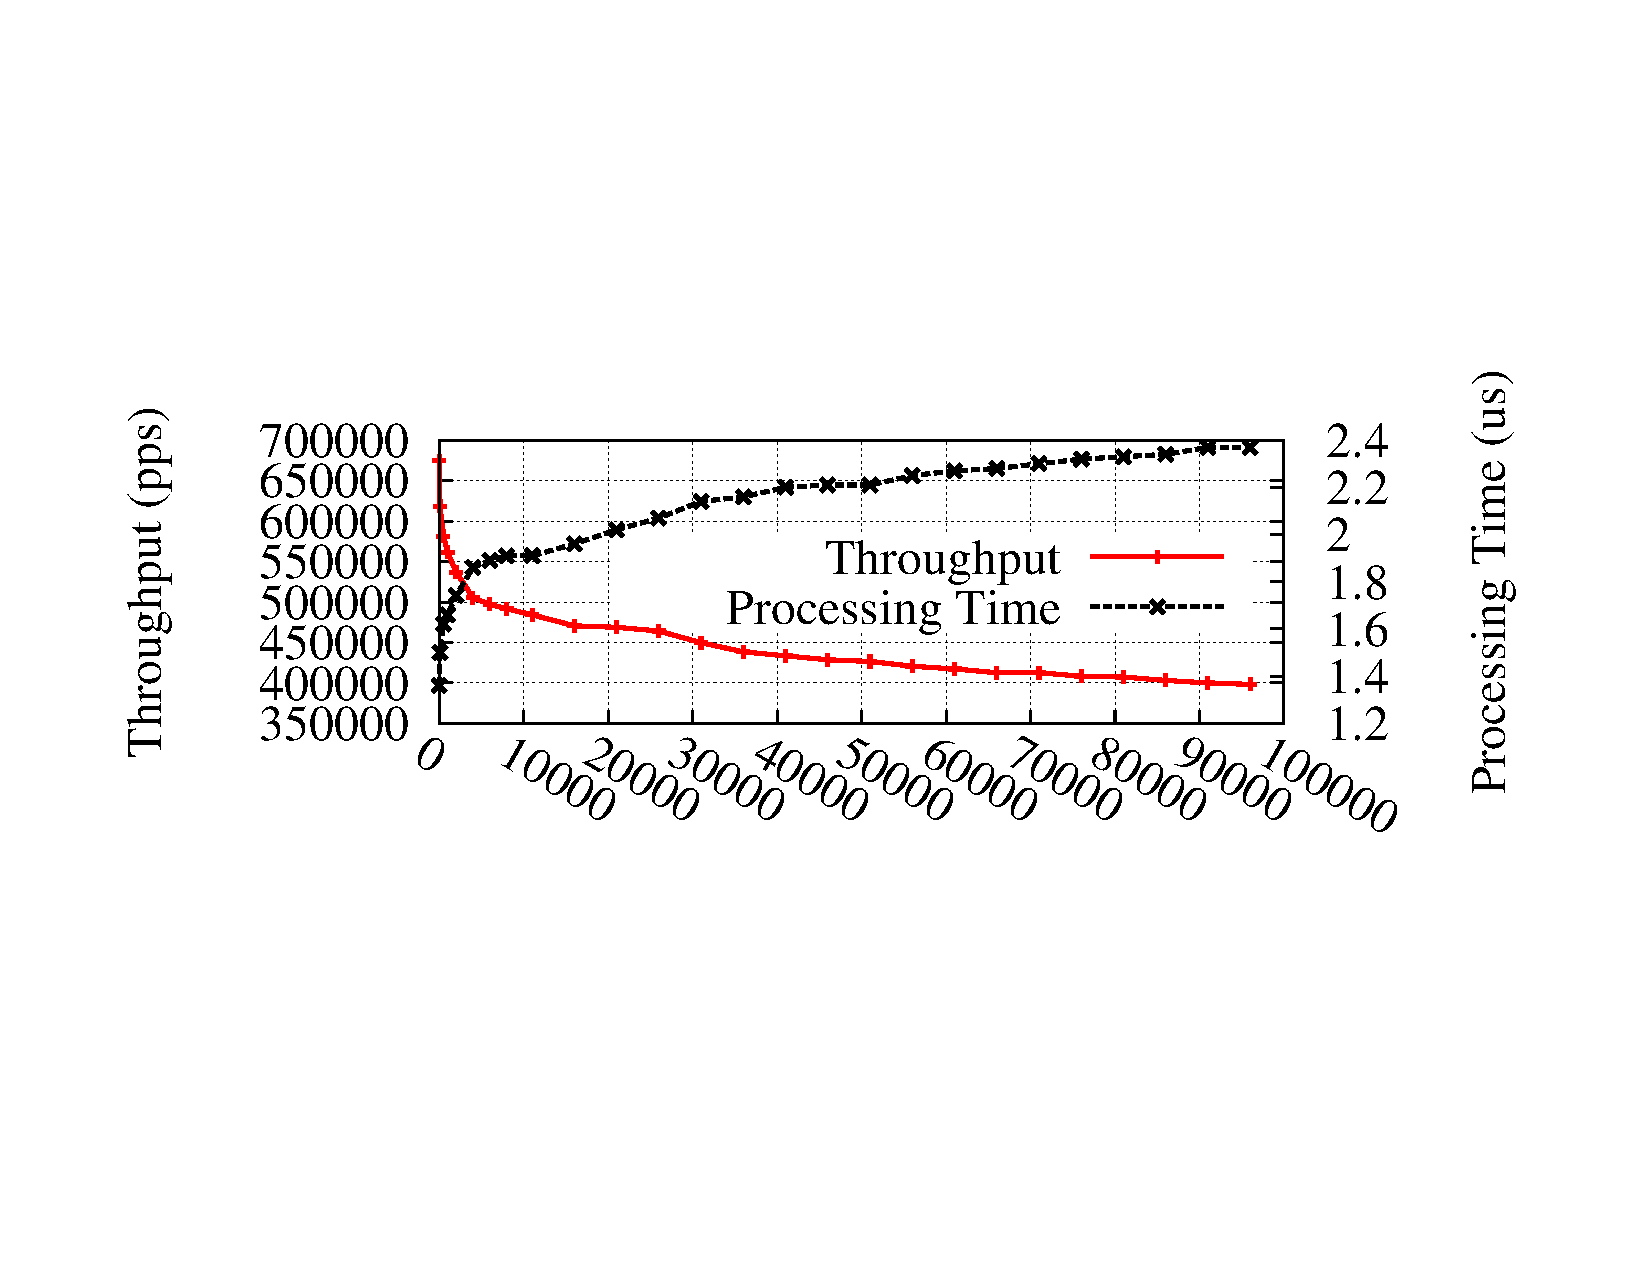
\includegraphics[width=3in]{fig/xputrange}
  \caption[]{\label{fig:xputrange} Throughput as \# of PrefixMatch rules increases.}
\end{figure}

\noindent{\it How do throughput and latency at the gateway scale with the number of rules for PrefixMatch?} 
In \S\ref{sec:range}, we discussed how PrefixMatch stores sorted intervals; every packet encryption requires a binary search of intervals. Hence, as the size of the tree goes larger, we can expect to require more time to process each packet and throughput to decrease. We measure this effect in Figure~\ref{fig:xputrange}. 
On the $y_1$ axis, we show the aggregate per packet throughput at the gateway as the number of rules from 0 to 100k. The penalty here is logarithmic, which is the expected performance of tree data structures. From 0-10k rules, throughput drops from 3Mpps to 1.5Mpps; after this point the performance penalty of additional rules tapers off. Adding an additional 90k rules drops throughput to 1.1Mpps.
On the $y_2$ axis, we measure the processing time per packet, \ie{}, the amount of time for the gateway to encrypt the packet; the processing time follows the same logarithmic trend.

\noindent{\it Is PrefixMatch faster than existing order preserving algorithms?}
PrefixMatch is the only encryption scheme that has low latency and the ordering property needed for packet processing.
We compare against BCLO~\cite{boldyreva:ope} and mOPE~\cite{popa:mope} below:

\begin{table}[h]
\vspace{-10pt}
\centering
\small
\begin{tabular}{c|c|c|c}
{\bf Operation}&{\bf BCLO}&{\bf mOPE}&{\bf \sys}\\
\hline
\hline
Encrypt, 10K rules&9333$\mu$s&6640$\mu$s&0.53$\mu$s\\
\hline
Encrypt, 100K rules&9333$\mu$s&8300$\mu$s&0.77$\mu$s\\
\hline
Decrypt&169$\mu$s&0.128$\mu$s&0.128$\mu$s\\
\hline
\end{tabular}
\vspace{-10pt}
\end{table}

\noindent{\it What is the memory overhead of PrefixMatch?}
Storing 10k rules in memory requires 1.6MB, and storing 100k rules in memory requires 28.5MB -- using unoptimized C++ objects.
This overhead is negligible.% on any modern server.

\subsubsection{Client Performance}

\begin{figure}
  \vspace{-10pt}
  \hspace{-15pt}
%  \begin{tabular}{cccc}
%  
\includegraphics[height=1in]{fig/cdflabel}
%  &\hspace{-10pt}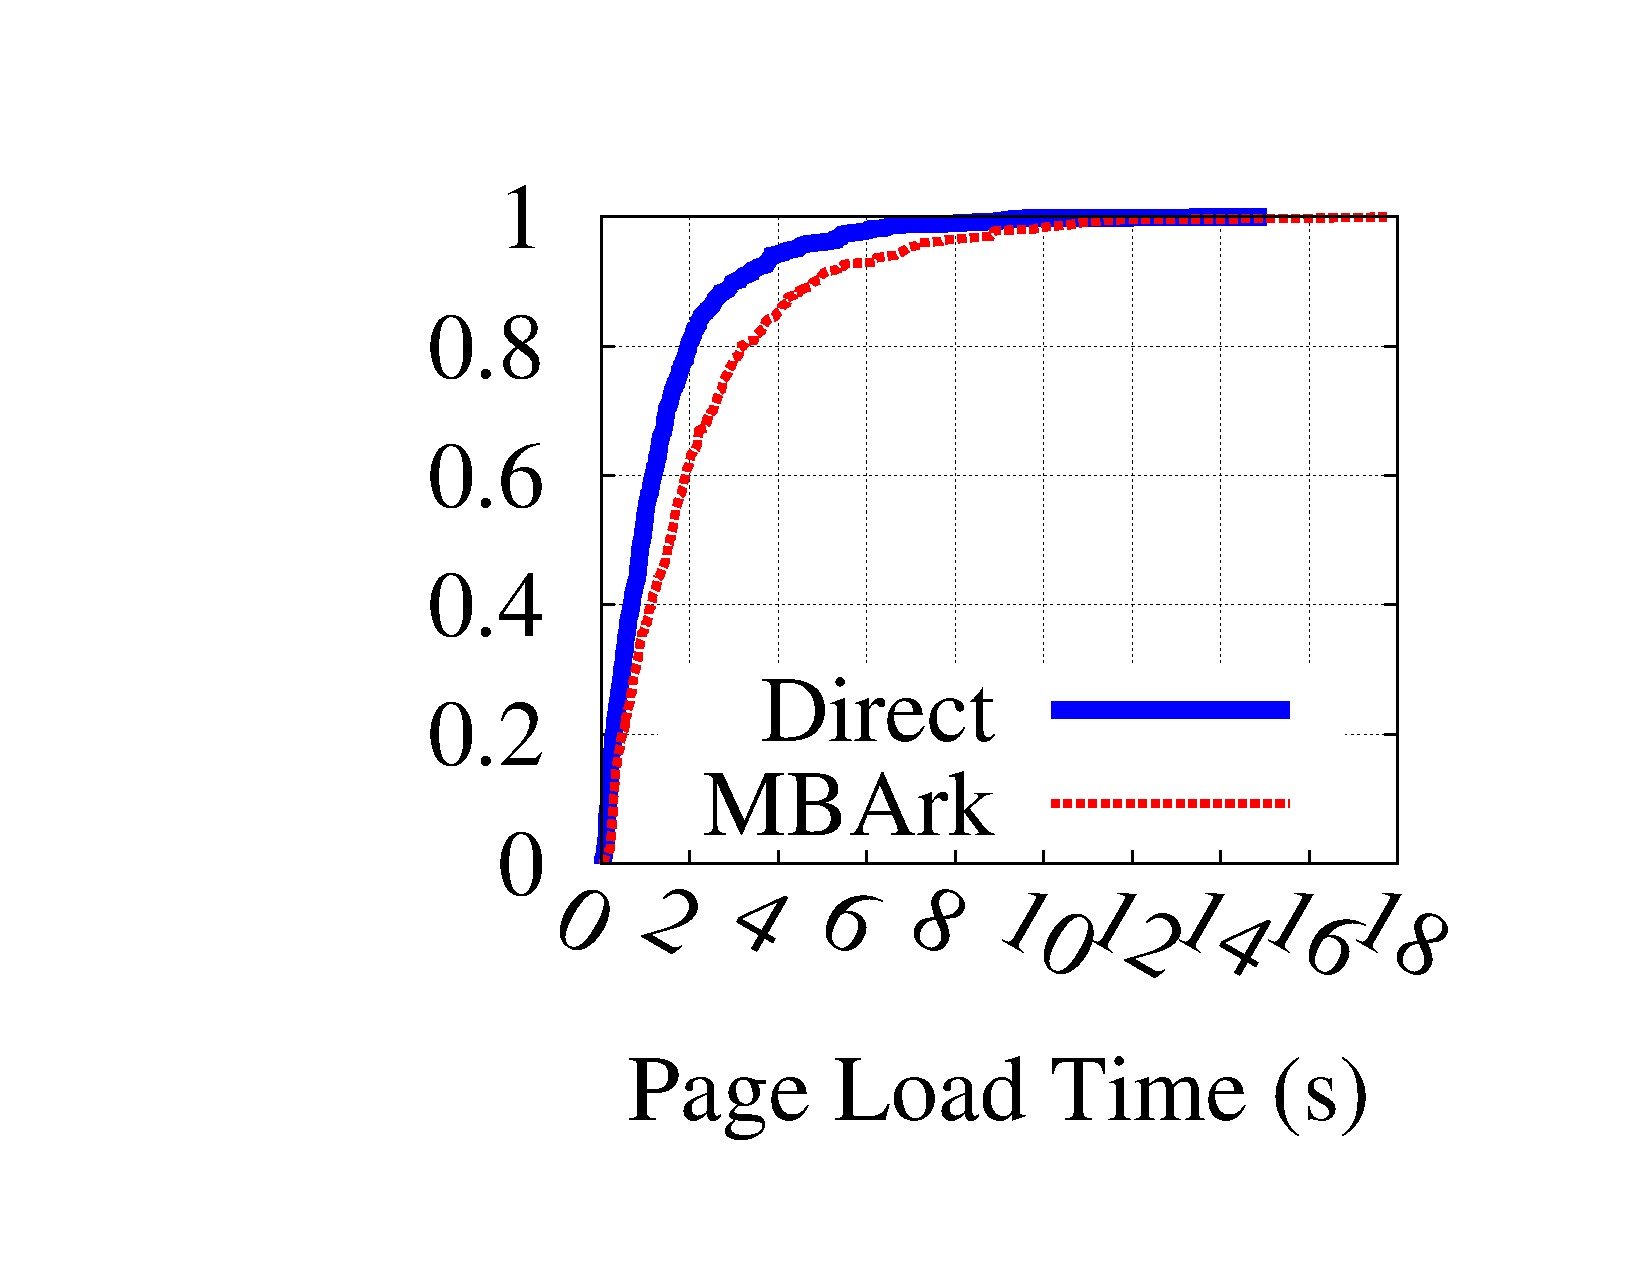
\includegraphics[height=.9in]{fig/e2e_loadtimes}
%  &\hspace{-10pt}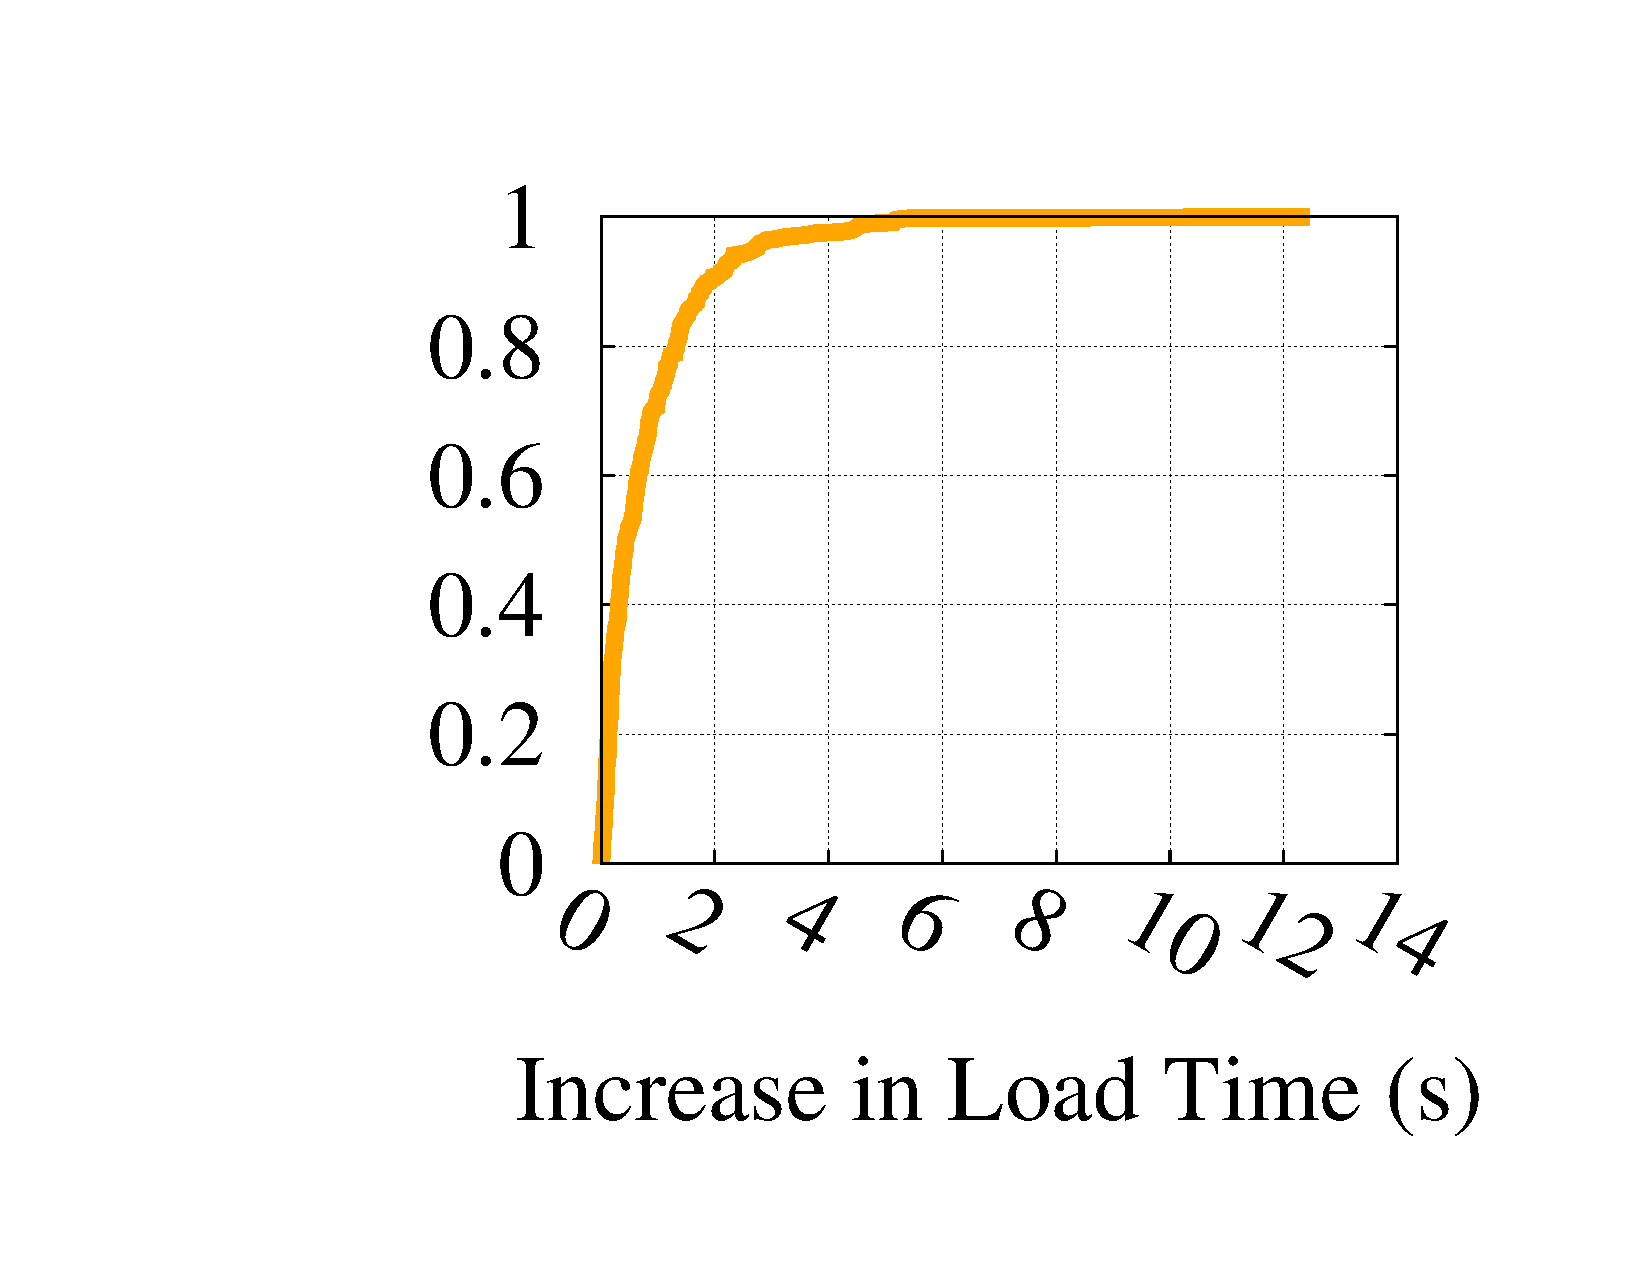
\includegraphics[height=.9in]{fig/e2e_delta_absolute}
%  &\hspace{-10pt}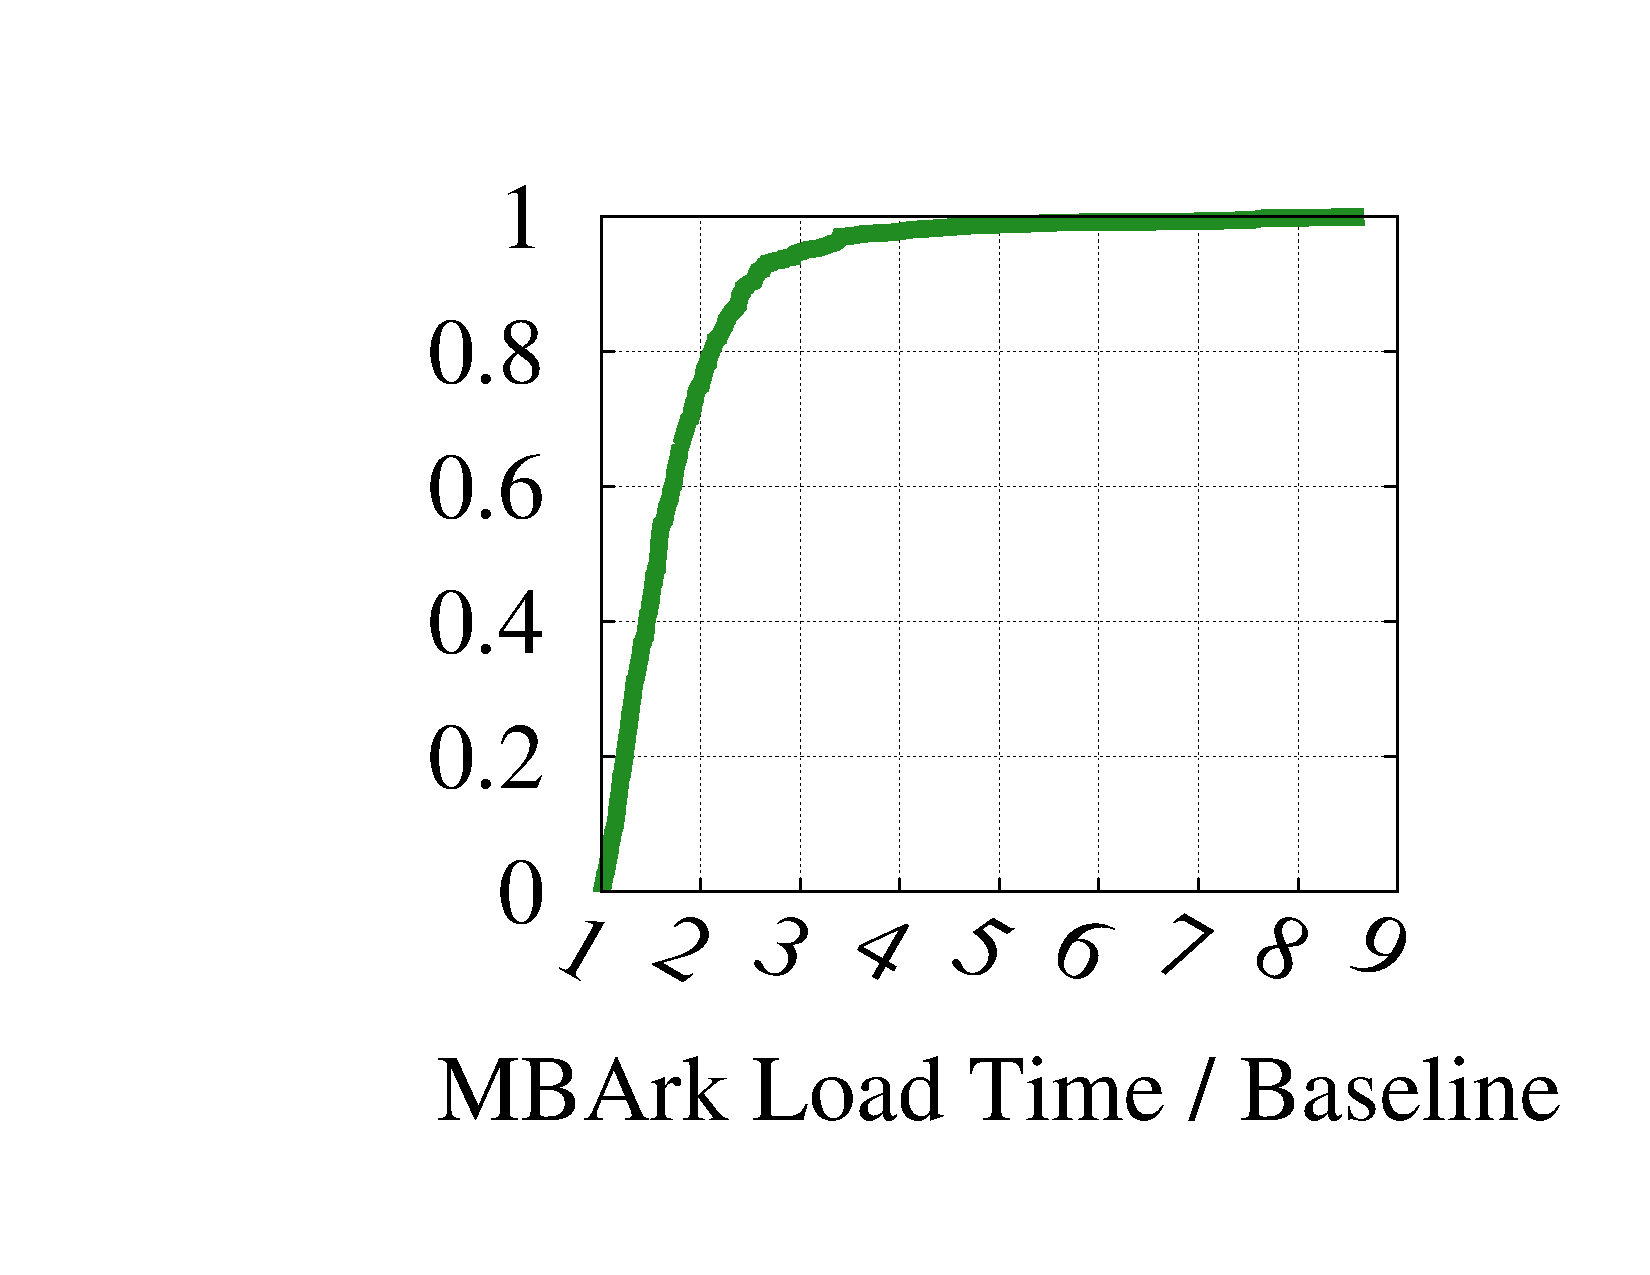
\includegraphics[height=.9in]{fig/e2e_delta_relative}
%  \\
%  &(a)&(b)&(c)\\
%  \end{tabular}
  \centering
  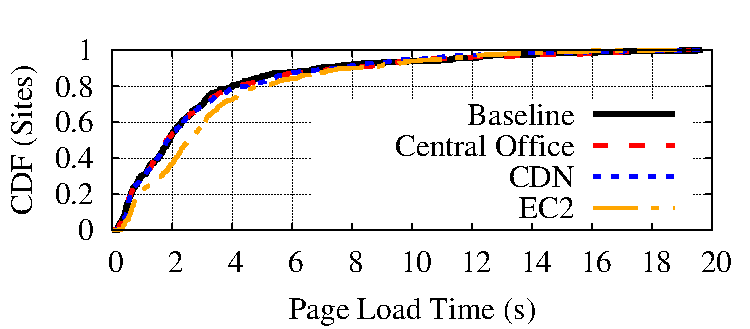
\includegraphics[width=2.7in]{fig/e2e_compare}
  \caption[]{\label{fig:e2eloads} Page load times under different deployments.}
\end{figure}

We use web performance to understand end-to-end user experience of \sys.
Figure~\ref{fig:e2eloads} shows a CDF for the Alexa top-500 sites loaded through our testbed. We compare the baseline (direct download) assuming three different service providers: an ISP hosting services in a Central Office (CO), a Content-Distribution Network, and a traditional cloud provider (EC2). The mean RTTs from the gateway are 60$\mu$s, 4ms, and 31ms, respectively. We deployed \sys on EC2 and used this deployment for our experiments, but for the CO and CDN we emulated the deployment with inflated latencies and servers in our testbed. We ran a pipeline of NAT, firewall and proxy (with empty cache) in the experiment.
Because of the `bounce' redirection \sys uses, all page load times increase by some fraction; in the median case this increase is less than 50ms for the ISP/Central Office, 100ms for the CDN, and 720ms using EC2; hence ISP based deployments will escape human perception~\cite{millishumans} but a CDN (or a cloud deployment) may introduce human-noticeable overheads.

\subsubsection{Bandwidth Overheads}
We evaluate two costs: the increase in bandwidth due to our encryption and metadata, and the increase in bandwidth cost due to `bounce' redirection.

\noindent{\it How much does \sys encryption increase the amount of data sent to the cloud?}
The gateway inflates the size of traffic due to three encryption costs:
\begin{myitemize}
  \item If the enterprise uses IPv4, there is a 20-byte per-packet cost to convert from IPv4 to IPv6. If the enterprise uses IPv6 by default, there is no such cost.
  \item If HTTP proxying is enabled, there are on average 132 bytes per request in additional encrypted data.
  \item If HTTP IDS is enabled, there is at worst a 5$\times$ overhead on all HTTP payloads~\cite{blindbox}.
\end{myitemize}
We used the m57 trace to understand how these overheads would play out in aggregate for an enterprise.
On the uplink, from the gateway to the middlebox service provider, traffic would increase by 2.5\% due to encryption costs for a header-only gateway. Traffic would increase by 4.3$\times$ on the uplink for a gateway that supports DPI middleboxes. 

\noindent{\it How much does bandwidth increase between the gateway and the cloud from using \sys? How much would this bandwidth increase an enterprises networking costs?}
\sys sends all network traffic to and from the middlebox service provider for processing, before sending that traffic out to the Internet at large. 

In ISP contexts, the clients' middlebox service provider and network connectivity provider are one and the same and one might expect costs for relaying the traffic to and from the middleboxes to be rolled in to one service `package;' given the latency benefits of deployment at central offices (as we saw in Fig.~\ref{fig:e2eloads}) we expect that ISP-based deployments are the best option to deploy \sys.

In the cloud service setting the client must pay a third party ISP to transfer the data to and from the cloud, before paying that ISP a third time actually transfer the data over the network.
Using current US bandwidth pricing~\cite{comcast-costs, megapath-costs, verizon-costs}, we can estimate how much outsourcing would increase overall bandwidth costs.
Multi-site enterprises typically provision two kinds of networking costs: Internet access, and intra-domain connectivity. 
Internet access typically has high bandwidth but a lower SLA; traffic may also be sent over shared Ethernet~\cite{comcast-costs, verizon-costs}.
Intra-domain connectivity usually has a private, virtual Ethernet link between sites of the company with a high SLA and lower bandwidth.
Because bounce redirection is over the `cheaper' link, the overall impact to bandwidth cost with header-only encryption given public sales numbers is between 15-50\%; with DPI encryption this cost increases to between 30-150\%. 

\eat{Getting frustrated with these numbers so leaving them here and will come back to them. Megapath offers a dedicated link at 5x5Mbps for \$250/mo; 20x20Mbps for \$1300/mo. Comcast offers enterprise cable at 150/20Mbps for \$250/mo. The three way bounce should result in a cost increase of 15-50\%, depending on how much the internal link is provisioned for. The DPI should be 2-3 times that, so, between 30-150\%... 
}

\subsection{Middleboxes}
\label{sec:evalcloud}

We now evaluate the overheads at each middlebox. 

\begin{table}[t!]
\small
\begin{tabular}{p{2.5cm}|p{2cm}|p{2cm}}
{\bf Application} &  {\bf Baseline Throughput} & {\bf \sys Throughput} \\
\hline \hline
IP Firewall &  9.8Gbps &  9.8Gbps \\
%Application Firewall  & & \\
NAT & 3.6Gbps   &   3.5 Gbps \\
%IP Forwarding  & & \\
%VPN Gateway &  &  &  \\ 
Load Balancer L4  &9.8 Gbps & 9.8Gbps \\
%Load Balancer L7 & & & \\
%WAN optimizer  & & & \\
Web Proxy &1.1Gbps &1.1Gbps\\
%IDS & & & \\
IDS & 85Mbps & 166Mbps~\cite{blindbox}   \\
\end{tabular}
\caption{Middlebox throughput for an empirical workload. \label{tbl:appsxput}}
\end{table}

\noindent{\it Is throughput reduced at the middleboxes due to  \sys?}

Table~\ref{tbl:appsxput} shows the throughput sustained for the apps we implemented.
The IP Firewall, NAT, and Load Balancer are all `header only' middleboxes; the results shown compare packet processing over the same dataplane, once with encrypted IPv6 data and once with unencrypted IPv4 data.
The only middlebox for which any overhead is observable is the NAT -- and this is a reduction of only 2.7\%.

We re-implemented the Web Proxy and IDS to enable the bytestream aware operations they require over our encrypted data. We compare our Web Proxy implementation with Squid~\cite{squid}. The Web Proxy sustains the same throughput with and without encrypted data, but, as we will present later, does have a higher service time per cache hit.
The IDS numbers compare Snort (baseline) to the BlindBox implementation; this is not an apples-to-apples comparison as BlindBox performs mostly exact matches where Snort matches regular expressions.

In what follows, we provide some further middlebox-specific benchmarks for the firewall, proxy, and IDS.

\noindent{\bf Firewalls:} 
{\it Does \sys support all rules in a typical firewall configuration? How much does the ruleset ``expand'' due to encryption?}

We tested our firewall with three rulesets provided to us by a network administrator at our institution and an IP firewall ruleset from Emerging Threats~\cite{emergingthreats}. We were able to encode all rules using range and keyword match encryptions. The size of 3 rulesets did not change after encryption, while the size of the other ruleset from Emerging Threats expanded from 1363 to 1370 -- a 0.5\% increase. Therefore we conclude that it has negligible impact on the firewall performance.


% We also investigated how much the ruleset increased due to PrefixMatch. Rules are typically encoded in the firewall as prefixes, hence a rule over the range [4.0.0.0, 4.255.255.255] is in practice implemented as a bit-mask over the first 8 bits of every packet. Using PrefixMatch, the same prefix might be mapped to 9.128.0.0-10.128.0.0.0, resulting in two /9 prefix ranges in the final rule encoding: 9.128.0.0/9 or 10.128.0.0/9. As throughput for many middleboxes decreases with the number of rules, we were concerned that these mappings might degrade performance. However, in practice rules increased modestly, by between 5.8\% and 10.2\%.

\begin{figure}[t]
\centering
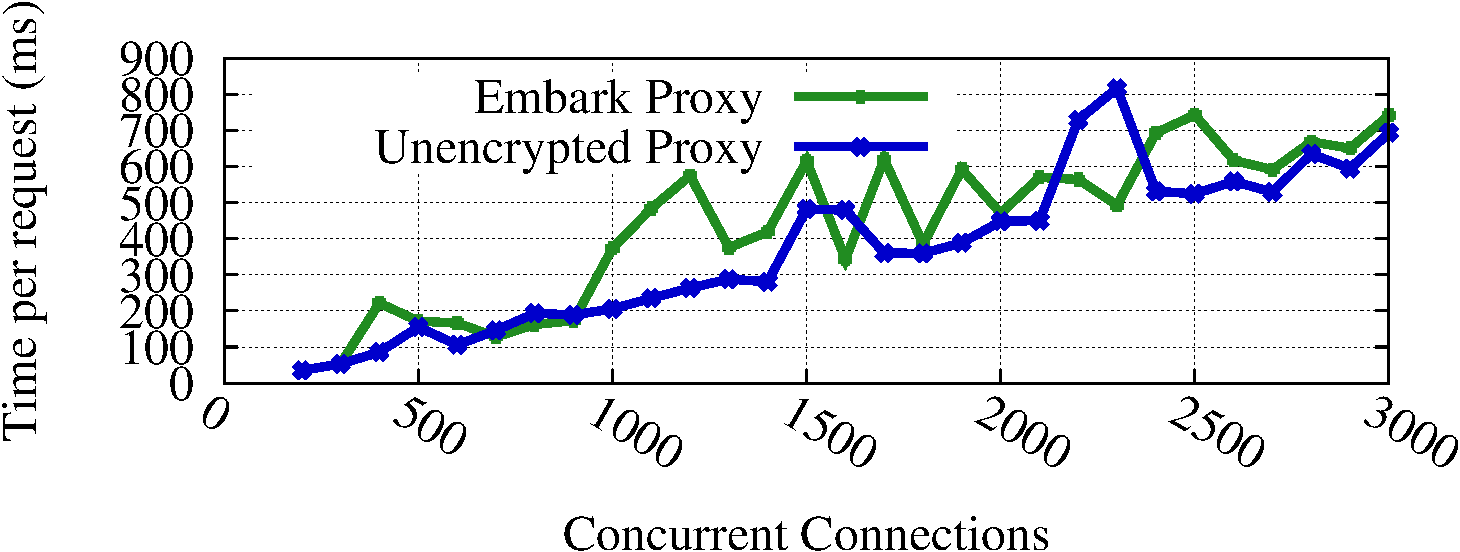
\includegraphics[width=3in]{fig/proxytime}
\caption{\label{fig:proxygraph} Access time per page against the number of concurrent connections at the proxy.}
\end{figure}

\noindent{\bf Proxy/Caching:} The throughput number shown in Table~\ref{tbl:appsxput} is not the typical metric used to measure proxy performance. A better metric for proxies is how many connections the proxy can handle concurrently, and what time-to-service it offers each client. In Figure~\ref{fig:proxygraph}, we plot time-to-service against the number of concurrent connections, and see that it is on average higher for \sys than the unencrypted proxy, by tens to hundreds of milliseconds per page.
This is not due to computation costs, but instead, due to the fact that the encrypted HTTP header values are transmitted on a different channel than the primary data connection.
The \sys proxy needs to synchronize between these two flows; this synchronization cost is what increases the time to service. 


\noindent{\bf Intrusion Detection:}
Our IDS is based on BlindBox~\cite{blindbox}. BlindBox incurs a substantial `setup cost' every time a client initiates a new connection. With \sys, however, the gateway and the cloud maintain one, long-term persistent connection. 
Hence, this setup cost is paid once when the gateway is initially configured. \sys also heuristically expands regular expressions in the rulesets into exact match strings. This results in two benefits:

\noindent{\it (1) End-to-end performance improvements.} Where BlindBox incurs an initial handshake of 414s~\cite{blindbox} to open a new connection, clients under \sys never pay this cost; instead they perform a normal TCP or SSL handshake of only 3-5 RTTs. In our testbed, this amounts to between 30 and 100 ms, depending on the site and protocol -- an improvement of 4 orders of magnitude.

\noindent{\it (2) Security improvements.} 
Using IDS rulesets from Snort, we converted regular expressions to exact match strings as discussed in \S\ref{sec:bbarch}. With 10G memory, we were able to convert about half of all regular expressions to a finite number of exact match strings; the remainder resulted in too many possible states. 
We used two rulesets to evaluate this~\cite{emergingthreats, snort-community}. With the first ruleset BlindBox would resort to the lower security level for 33\% of rules, but \sys would only require this for 11.3\%. With the second ruleset, BlindBox would use lower security for 58\% of rules, but \sys would only do so for 20.2\%. The major drawback of \sys is that \sys cannot perform probable cause encryption, because there is no end-to-end SSL session in the \sys scenario. However, \sys still strictly improves the security in this outsourcing scenario.

\eat{
\begin{table}[h]
  \centering
  \small
  \begin{tabular}{l|c|c}
  %\begin{tabular}{p{1.75in}|p{.4in}|p{.4in}}
    {{\bf Rule Set}}&{\bf Exact Match}&{\bf Prob. Cause}\\
    \hline
    \hline
    BB: Community&67\%&100\%\\
    \hline
    MB: Community&88.7\%&100\%\\

    \hline
    \hline
    BB: Emerging Threats&42\%&100\%\\
    \hline
    MB: Emerging Threats&79.8\%&100\%\\
    \hline
  \end{tabular}
\end{table}
}

